%=================
%     PACKAGES
%=================
\usepackage{graphicx,latexsym}
\usepackage{amssymb,amsthm,amsmath}
\usepackage{physics}
\usepackage{longtable,booktabs,setspace}
\usepackage[hyphens]{url}
\usepackage{rotating}
\usepackage{natbib}
\usepackage{euscript}
\usepackage{dsfont} % Boldface 1 for indicator function
\usepackage{array} % For the analytical eigenvector proof (block matrices)
% \usepackage{times} % other fonts are available like times, bookman, charter, palatino

% For arrows with text on them
\usepackage{mathtools}

% For the quote environments!
\usepackage[utf8]{inputenc}
\usepackage{epigraph}

% For code snippet environments
\usepackage{listings}
\usepackage[svgnames]{xcolor}

%=============================
%     THEOREM ENVIRONMENTS
%=============================
% Theorems
\newtheorem{theorem}{Theorem}[section]
\setlength{\parskip}{0pt}
\setlength\parindent{24pt}

% Defintions
\newtheorem{definition}{Definition}[section]
\setlength{\parskip}{0pt}
\setlength\parindent{24pt}

% Examples
\newtheorem*{example}{Example}
%\newtheorem{example}{Example}[section]
\setlength{\parskip}{0pt}
\setlength\parindent{24pt}

% Code Examples
\newtheorem*{code}{Code Example}
%\newtheorem{code}{Code Example}[section]
\setlength{\parskip}{0pt}
\setlength\parindent{24pt}

% Notes
\newtheorem*{note}{Note}
%\newtheorem{note}{Note}[section]
\setlength{\parskip}{0pt}
\setlength\parindent{24pt}

% Algorithms
\newtheorem{algorithm}{Algorithm}[section]
\setlength{\parskip}{0pt}
\setlength\parindent{24pt}

% Algorithms (unnumbered)
\newtheorem*{algorithm*}{Algorithm}%[section]
\setlength{\parskip}{0pt}
\setlength\parindent{24pt}

% Remarks
\newtheorem*{remark}{Remark}
%\newtheorem{remark}{Remark}[section]
\setlength{\parskip}{0pt}
\setlength\parindent{24pt}

% Formalization
\newtheorem*{formalization}{Formalization}
\setlength{\parskip}{0pt}
\setlength\parindent{24pt}

% Warning
\newtheorem*{warning}{Warning}
\setlength{\parskip}{0pt}
\setlength\parindent{24pt}

%=====================
%     ENVIRONMENTS
%=====================
\usepackage{tcolorbox}
% Blue box
\definecolor{bbxcolor}{RGB}{0,60,255}% Rule colour
\newtcbox{\bbx}{on line,
  colframe=bbxcolor,colback=bbxcolor!10!white,
  boxrule=0.5pt,arc=4pt,boxsep=0pt,left=6pt,right=6pt,top=6pt,bottom=6pt}
%=====================
% Red box
\definecolor{rbxcolor}{RGB}{190,30,45}
\newtcbox{\rbx}{on line,
  colframe=rbxcolor,colback=rbxcolor!10!white,
  boxrule=0.5pt,arc=4pt,boxsep=0pt,left=6pt,right=6pt,top=6pt,bottom=6pt}
%=====================
% R Code Chunks
\lstset{language=R,
    basicstyle=\small\ttfamily,
    stringstyle=\color{DarkGreen},
    otherkeywords={0,1,2,3,4,5,6,7,8,9},
    morekeywords={TRUE,FALSE},
    deletekeywords={data,frame,length,as,character},
    keywordstyle=\color{blue},
    commentstyle=\color{DarkGreen},
}
\xdefinecolor{gray}{rgb}{0.4,0.4,0.4}
\xdefinecolor{blue}{RGB}{58,95,205}% R's royalblue3; #3A5FCD
%=====================
%% Single quotation environment for introduction
\def\signed #1{{\leavevmode\unskip\nobreak\hfil\penalty50\hskip2em
  \hbox{}\nobreak\hfil(#1)%
  \parfillskip=0pt \finalhyphendemerits=0 \endgraf}}

% Quote environment
\newsavebox\myqbox
\newenvironment{aquote}[1]
  {\savebox\myqbox{#1}\begin{quote}}
  {\signed{\usebox\myqbox}\end{quote}}
%=====================


%==================
%     FORMAT
%==================
% Mini title document environment
\newcommand{\minititle}[1]{
  \begin{center}
    \textbf{#1}
  \end{center}
}

\newcommand{\blocktitle}[1]{ \noindent \textbf{#1.}}

\newcommand{\trim}{\vspace{-1em}}
\newcommand{\trimm}{\vspace{-2em}}
\newcommand{\trimmm}{\vspace{-3em}}
%==================
%     COMMANDS
%==================
% Latin Letters (bb)
\newcommand{\Cc}{\mathbb{C}} % Complex Numbers
\newcommand{\R}{\mathbb{R}} % Reals
\newcommand{\N}{\mathbb{N}} % Naturals
\newcommand{\F}{\mathbb{F}} % Field

% Latin Letters (cal)
\newcommand{\B}{\mathcal{B}} % Batch
\newcommand{\Rseq}{\mathcal{R}} % Ratio-Sequence
\newcommand{\Seq}{\mathcal{S}} % Sequence
\renewcommand{\S}{\mathbb{S}} % Spectrum
\newcommand{\Ens}{\mathcal{E}} % Ensemble
\newcommand{\D}{\mathcal{D}} % Distribution

% Greek letters
\renewcommand{\epsilon}{\varepsilon}
\newcommand{\ep}{\epsilon}
\renewcommand{\d}{\delta}
\renewcommand{\b}{\beta}

% Probability & Probability Distributions
\newcommand{\Prb}{\text{P}}
\newcommand{\E}{\mathbb{E}}
\newcommand{\Var}{\text{Var}}
\newcommand{\Unif}{\text{Unif}}
\newcommand{\Bern}{\text{Bern}}
\newcommand{\Bin}{\text{Bin}}
\newcommand{\Normal}{\mathcal{N}}

% Math macros
\newcommand{\oneto}[1][n]{1,\dots,#1} % 1,...,n
\newcommand{\sumi}[1][n]{\sum_{i = 1}^{#1}} % sum from i = 1 to n
\newcommand{\seq}[2][n]{{{#2}_0,{#2}_1,\dots,{#2}_{#1}}} % x_1,...,x_n

% Words
\newcommand{\where}{\text{ where }}
\newcommand{\for}{\text{ for }}
\newcommand{\given}{\text{ given }}
\renewcommand{\and}{\text{ and }}

% Other
\newcommand{\ra}{\rightarrow}

%==================
%     TABLES
%==================
%============================
%      D-DISTRIBUTIONS
%============================
\newcommand{\Ddisttable}{
  \begin{tabular}{ |p{3cm}||p{3cm}|p{3cm}|p{3cm}|  }
   \hline
   \multicolumn{4}{|c|}{Table of Random Matrix Distributions} \\
   \hline
   Distribution & Notation ($\D$) & Parameters & Class\\
   \hline
   Normal & $\Normal(\mu,\sigma)$ & $\mu \in \R, \sigma \in \R^+$  &  Explicit\\
   Uniform  & $\Unif(a,b)$ & $a,b \in \R$ & Explicit\\
   Hermite-$\beta$   & $\mathcal{H}(\beta)$  &  $\b \in \N$  & Implicit\\
   Erdos-$p$   &   $\text{ER}(p)$  & $p \in [0,1]$   & Implicit\\
   \hline
  \end{tabular}
}
%============================
%      SPECTRUM SCHEMES
%============================
\newcommand{\spectrumschemetable}{
  \begin{tabular}{ |p{3cm}||p{2cm}|p{2.5cm}|p{4.5cm}|  }
   \hline
   \multicolumn{4}{|c|}{Table of Spectrum Schema} \\
   \hline
   Scheme & Matrix & Notation & Ordering \\
   \hline
   Sign-Ordered & $P$ & $\sigma_{S}(P)$ & $\lambda_1 \geq \lambda_2 \geq ... \geq \lambda_N$ \\
   Norm-Ordered & $P$ & $\sigma_{N}(P)$ & $|\lambda_1| \geq |\lambda_2| \geq ... \geq |\lambda_N|$ \\
   Singular & $P \cdot P^T$ & $\sigma_{+}(P)$ & $\sqrt{\lambda_1} \geq \sqrt{\lambda_2} \geq ... \geq \sqrt{\lambda_N}$ \\
   \hline
  \end{tabular}
}
%============================
%     DISPERSION METRICS
%============================
\newcommand{\dispersiontable}{
  %\begin{tabular}{ |p{5cm}||p{2cm}|p{2cm}|p{2cm}|p{2cm}|  }
  \begin{tabular}{ |p{4.4cm}||p{1.9cm}|p{1.9cm}|p{1.9cm}|p{1.9cm}|  }
   \hline
   \multicolumn{5}{|c|}{Table of Dispersion Metrics} \\
   \hline
   Metric* & Notation & Formula & Symmetric & Parameters\\
   \hline
   Standard Norm & $\d$ & $|z' - z|$ &  True & - \\
   $\beta$-Norm & $\d_\b$ & $|z' - z|^\b$ & True & $\b \in \N$ \\
   Difference of Absolutes & $\d_{\text{abs}}$ & $|z'| - |z|$ &  False  &  - \\
   Identity Difference &  $\d_{\text{id}}$ & $z' - z$ & False &  - \\
   %Angola & AO & AGO & 024\\
   \hline
  \end{tabular}
}
%============================
%      PAIRING SCHEMES
%============================
\newcommand{\pairingschemetable}{
  %\begin{tabular}{ |p{2.5cm}||p{1.75cm}|p{5.5cm}|  }
  %\begin{center}
    \begin{tabular}{ |p{3cm}||p{3cm}|p{6cm}|  }
     \hline
     \multicolumn{3}{|c|}{Table of Pairing Schema} \\
     \hline
     Scheme & Notation & Formula \\
     \hline
     Lower & $\Pi_<$ & $\{(i,j) \mid i < j \for i,j \in \N_N \}$ \\
     Upper  & $\Pi_>$ & $\{(i,j) \mid i > j \for i,j \in \N_N \}$ \\
     Consecutive  & $\Pi_C$ & $\{(i,j) \mid i = j + 1 \for i,j \in \N_N \}$ \\
     All & $\Pi_0$ & $\{(i,j) \mid i,j \in \N_N \}$ \\
     \hline
    \end{tabular}
  %\end{center}
}


%==================
%     GRAPHICS
%==================
%==================
%     CHAPTER 2
%==================

\newcommand{\FIGUREspectrumcomparison}[2]{
  \begin{figure}[#1]
   \begin{center}
    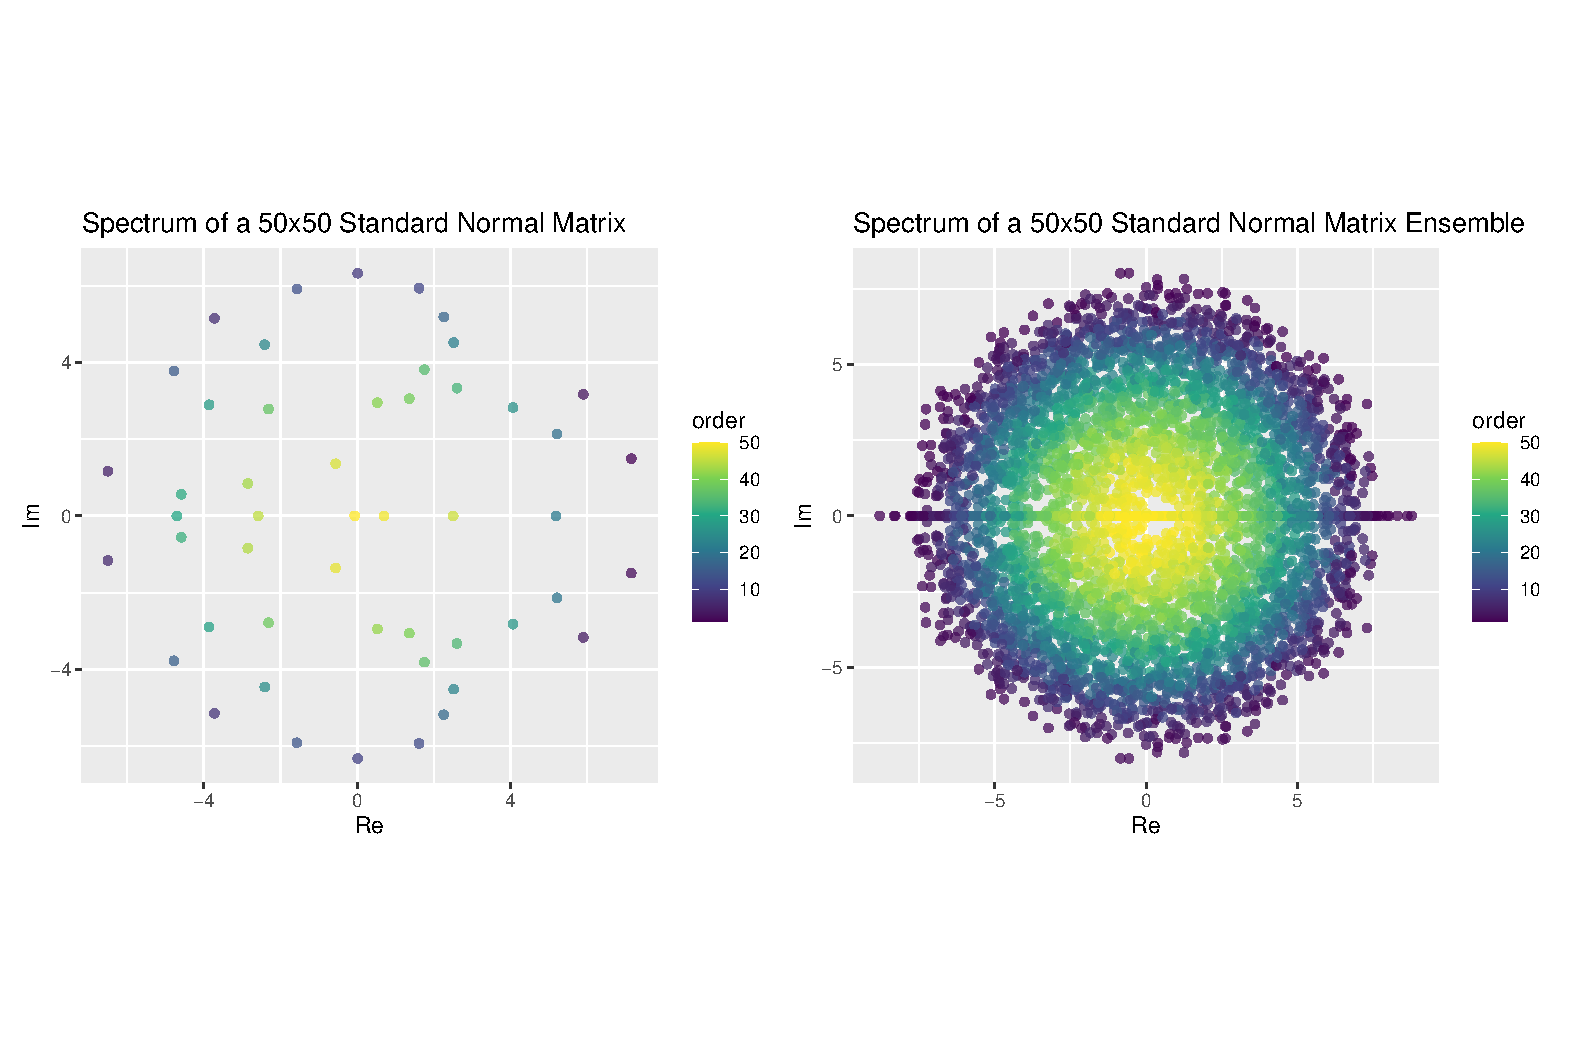
\includegraphics[scale = #2]{../graphics/chap2/2-1-2_comparison}
    \caption{Spectrum of a Matrix versus an Ensemble}
   \end{center}
   \label{ensemble_comparison_plot}
  \end{figure}
}

\newcommand{\FIGUREnormalspectrum}[2]{
  \begin{figure}[#1]
   \begin{center}
    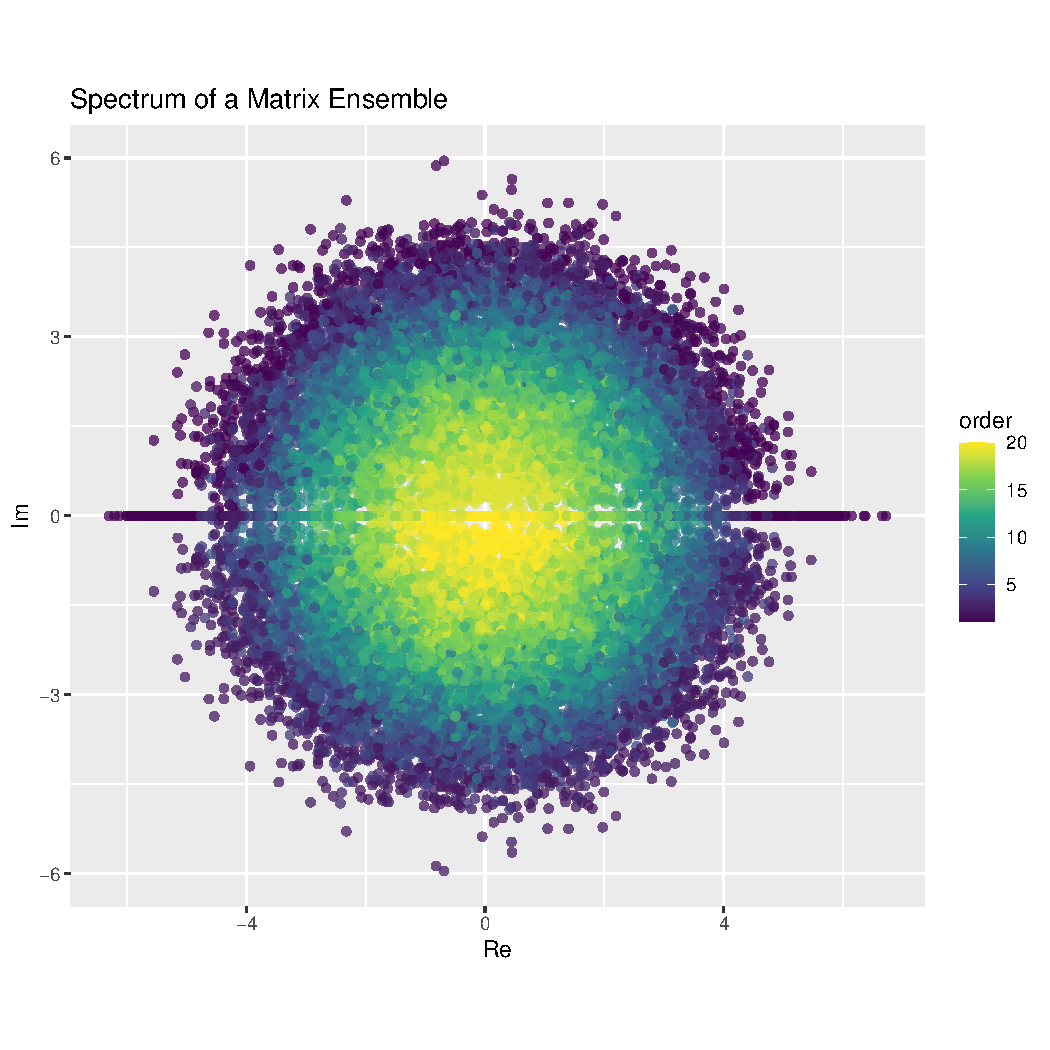
\includegraphics[scale = #2]{../graphics/chap2/2-1-2_normal_spec}
    \caption{Spectrum of a Standard Normal Matrix ensemble}
   \end{center}
   \label{spectrum_normal_ensemble_plot}
  \end{figure}
}

\newcommand{\FIGUREorderscheme}[2]{
  \begin{figure}[#1]
   \begin{center}
    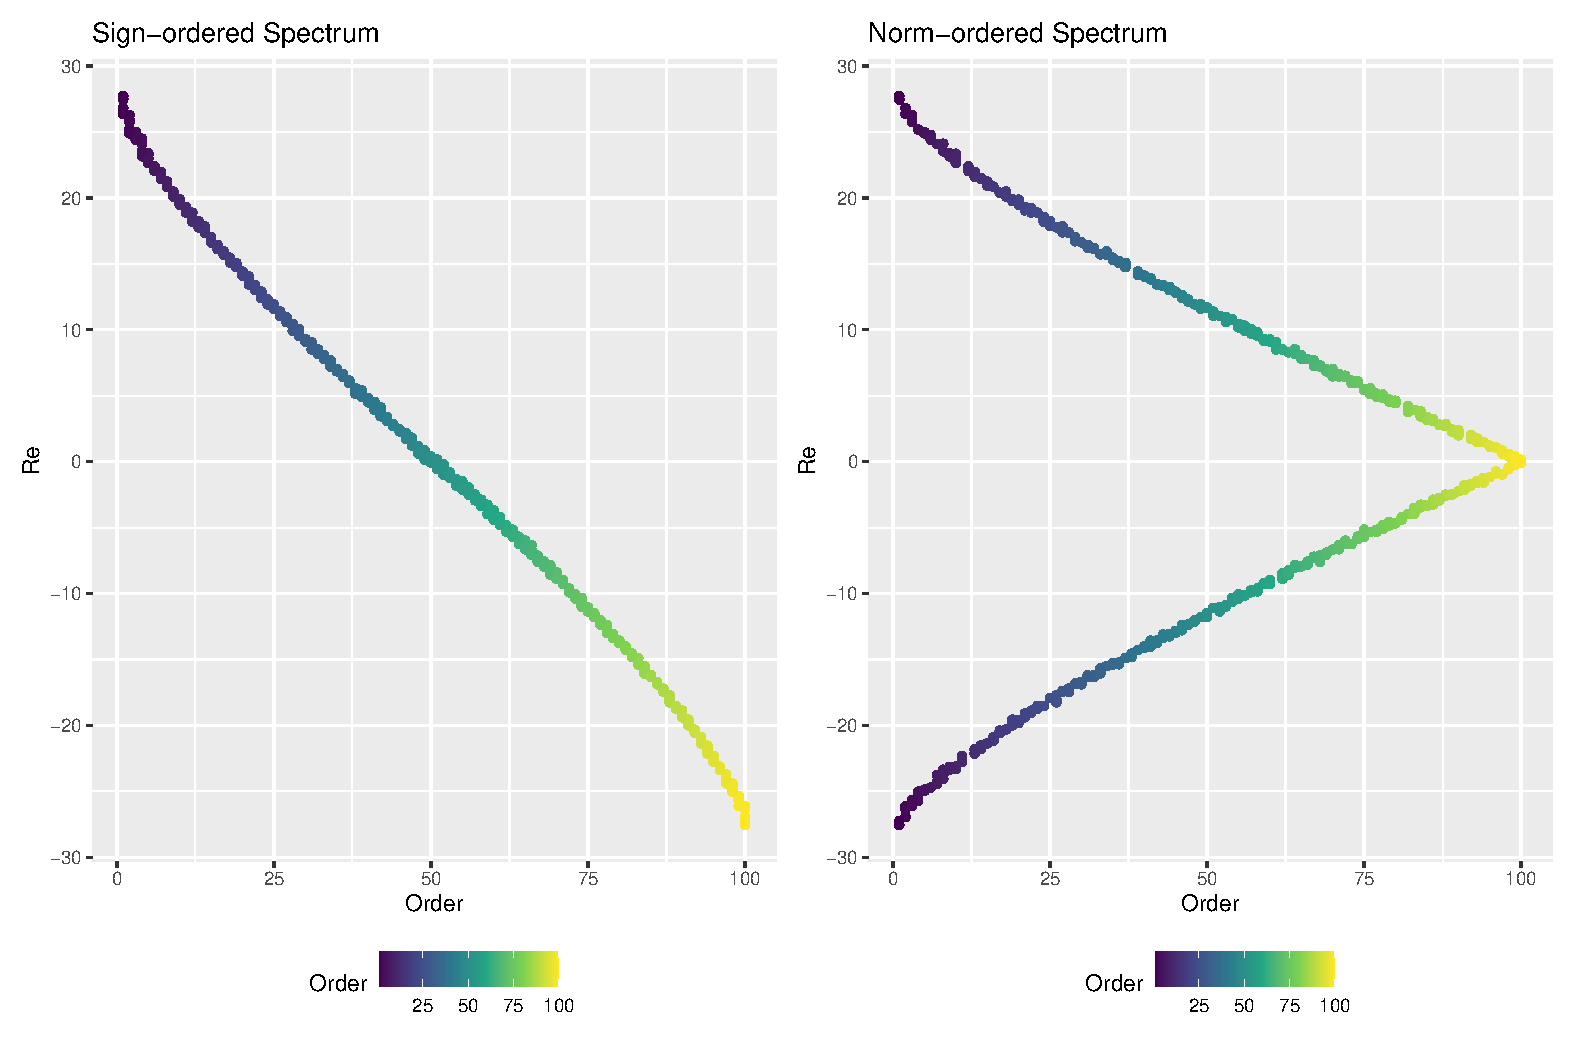
\includegraphics[scale = #2]{../graphics/chap2/2-2-1_orderscheme}
    \caption{Spectrum displaying two different ordering scheme}
   \end{center}
   \label{orderscheme_plot}
  \end{figure}
}

\newcommand{\FIGUREsemicircle}[2]{
  \begin{figure}[#1]
   \begin{center}
    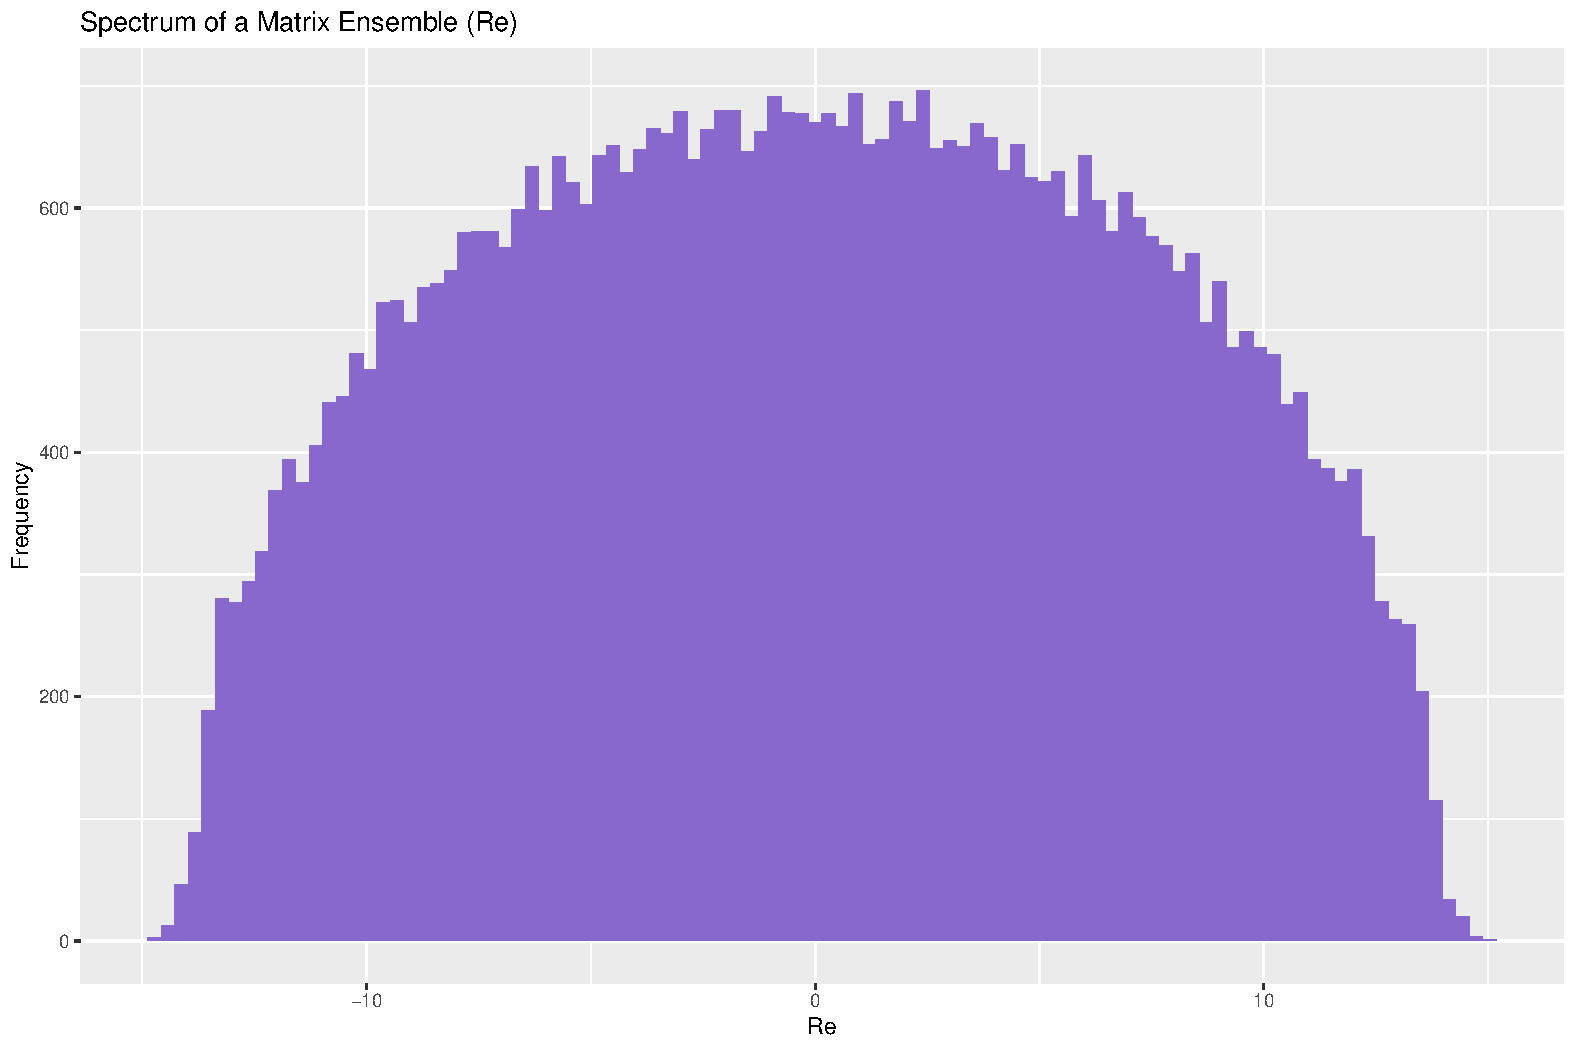
\includegraphics[scale = #2]{../graphics/chap2/2-3-2_semicircle}
    \caption{Eigenvalues of a Symmetric Matrix displaying the Semicircle Distribution}
   \end{center}
   \label{semicircleplot}
  \end{figure}
}
%==================
%     CHAPTER 3
%==================

%==================
%     CHAPTER 4
%==================s


%==================
%     PROOFS
%==================
%%%%%%%%%%%%%%%%%%%%%%%%%%%%%%%%%%%%%%%%%%%%%%%%%%%%
%                   LEMMA PROOF
%%%%%%%%%%%%%%%%%%%%%%%%%%%%%%%%%%%%%%%%%%%%%%%%%%%%
\newcommand{\lemmaproof}{
\blocktitle{Proof of Lemma} Begin by taking a real symmetric matrix $S_M$ for some $M \in \N$. Suppose we have an eigenvalue $\lambda$. Then, if we have some eigenvector $v$, we know that:
$$(1): \forall i \in \N_{M} : a_1v_1 + \dots + d_iv_i + \dots + a_{m-1}v_m = \lambda v_i \quad ( a_j \in \R)$$
We obtain $(1)$ by expanding the equality $A\vec{v} = \lambda \vec{v}$ and noticing that every row of $Av$ is expressible as the sum of the non-diagonal entries multiplied by $v_j \mid j \neq i$ plus $d_i v_i$.  % Note that since our matrix is symmetric, for some rows, some of the constants $a_j$ are not distinct but this should not raise any issues.
%%%%%%%%%%%%%%%%%%%%%%%%%%%%%%%%%%%%%%%%%%%%%%%%%%%%
Next, we collect the terms to solve for $v_i$:
$$\forall i \in \N_{M} : a_1v_1 + \dots + a_{m-1}v_m =  v_i(\lambda - d_i)$$
%%%%%%%%%%%%%%%%%%%%%%%%%%%%%%%%%%%%%%%%%%%%%%%%%%%%
Since $S_M$ is a real symmetric matrix, the $a_j$ terms are real so we can say:
$$\forall i \in \N_{M} :  v_i(\lambda - d_i) = \sum_{j \neq i} a_jv_j \quad (a_j \in \R)$$
Finally, divide both sides by $(\lambda - d_i)$. On the right hand side, the coefficients of $v_j$ become $\frac{a_j}{(\lambda - d_i)}$. Denote this coefficient ${a}'_j = \frac{a_j}{(\lambda - d_i)}$. %%%%%%%%%%%%%%%%%%%%%%%%%%%%%%%%%%%%%%%%%%%%%%%%%%%%
Since $S_M$ is a real symmetric matrix, we know its eigenvalues are real so $\lambda \in \R$ and that its entries are real so $a_i, d_i \in \R$.
\noindent Since ${a}'_j$ is an arithmetic expression involving real numbers, then it follows that for every $j$, ${a}'_j \in \R$. As such, we can rewrite $v_j$ as the following sum.
$$\forall i \in \N_{M}: v_i =  {\sum_{j \neq i} c_j v_j} \quad (\forall j: {a}'_j \in \R)$$
%%%%%%%%%%%%%%%%%%%%%%%%%%%%%%%%%%%%%%%%%%%%%%%%%%%%
Thus, for any $M \in \N$, a real symmetric matrix $S_M \in \R^{M \times M}$ with eigenvalue $\lambda$ must have a corresponding eigenvector $v$ such that each of its entries is expressible as a real linear combination of the other entries. So, the proof is complete. $\square$
}
%%%%%%%%%%%%%%%%%%%%%%%%%%%%%%%%%%%%%%%%%%%%%%%%%%%%
%                 THEOREM PROOF
%%%%%%%%%%%%%%%%%%%%%%%%%%%%%%%%%%%%%%%%%%%%%%%%%%%%
\newcommand{\taqiproof}{
\blocktitle{Proof} For this proof we will induct on the dimension of the matrix, $M$. So, let the inductive statement be:
$$f(M) : S_M\text{ has a real eigenvector } v \text{ corresponding to an eigenvalue } \lambda$$

%%%%%%%%%%%%%%%%%%%%%%%%%%%%%%%%%%%%%%%%%%%%%%%%%%%%
\blocktitle{Base Case} Take the base case $M = 2$. This proof is left to the reader as an exercise. Begin by taking a $2 \times 2$ symmetric matrix, and show that there exist real coefficients for the eigenvector corresponding to $\lambda$ by using Gaussian Elimination. \newline
%%%%%%%%%%%%%%%%%%%%%%%%%%%%%%%%%%%%%%%%%%%%%%%%%%%%

\blocktitle{Inductive Step} For our inductive step, we need to show that $f(M) \Rightarrow f(M+1)$. So, let us assume $f(M)$. This means that we can assume any real symmetric matrix $S_M$ has a real eigenvector $v \in \R^M$ corresponding to $\lambda$. \newline

%%%%%%%%%%%%%%%%%%%%%%%%%%%%%%%%%%%%%%%%%%%%%%%%%%%%
\noindent Next, we will write $S_{M+1}$ as the matrix $S_M$ augmented by some $u \in \R^M$ as follows:
$$ S_{M+1} =
\left[
  \begin{array}{c|c}
  S_M & u\\
  \hline
  u^T & d_{M+1}
\end{array} \right]$$
From our lemma, we use the fact that $S_{M+1}$ is symmetric and our lemma to obtain (1) and our assumption of $f(M)$ to obtain (2), listed below:
$$(1): \forall i \in \N_{M+1}: v_i =  {\sum_{j \neq i} c_j v_j} \quad (c_j \in \R)$$
$$(2): \forall i \in \N_{M}: v_i \in \R$$
In particular for $(2)$, we know that $v_i = \left({\sum_{j \neq i} \frac{a_j}{d_i-\lambda} v_j}\right)$.
%%%%%%%%%%%%%%%%%%%%%%%%%%%%%%%%%%%%%%%%%%%%%%%%%%%%
From (1), we know that for the $(m+1)^{th}$ row, $v_{m+1} =  {\sum_{j \neq {m+1}} c_j v_j}$ for real coefficients $c_j \in \R$. By (2), this is a linear combination of real entries $v_i$. Since $v_{m+1} \in \R$, this means we have shown that:
$$\forall i \in \N_{M+1}: v_i \in \R$$
%%%%%%%%%%%%%%%%%%%%%%%%%%%%%%%%%%%%%%%%%%%%%%%%%%%%
In other words, we have established that $f(M) \Rightarrow f(M+1)$. By induction, the proof of the theorem is complete. $\square$.
}


%==================
%    ALGORITHS
%==================

%%%%%%%%%%%%%%%%%%%%%%%%%%%%%%%%%%%%%%%%%%%%%%%%%%%%%%%%%%%%%%%%%%%%%%%%%%%%%%%%%%%%%%%%%%%%%%%%
% 																	Implicit D-Matrices
%%%%%%%%%%%%%%%%%%%%%%%%%%%%%%%%%%%%%%%%%%%%%%%%%%%%%%%%%%%%%%%%%%%%%%%%%%%%%%%%%%%%%%%%%%%%%%%%

\newcommand{\ALGstochrow}{
	\begin{algorithm}[Stochastic Row] \hfill
	\begin{enumerate}
		\item To sample a row $r$ of size $N$, fix $N \in \N$.
		\item Sample a vector $\vec{X}$ with $N$ i.i.d entries between $[0,1]$. So, sample $\vec{X} \sim \Unif(0,1)$.
		\item Assign $r \la \vec{X}$, and then normalize the row by diving each entry by the row sum; so assign $r \la r \cdot \frac{1}{\sum_{i = 1}^N{r_i}}$
		\item Return the stochastic row $r$.
	\end{enumerate}
	\end{algorithm}
}

\newcommand{\ALGstoch}{
	\begin{algorithm}[Stochastic Matrix] \hfill
	\begin{enumerate}
		\item To generate a stochastic square matix $P$ of size $N$, fix $N \in \N$.
		\item Then, for every row of $P$, randomly sample a stochastic row and assign it to $P$.
		\item Return the stochastic matrix $P$.
	\end{enumerate}
	\end{algorithm}
}

\newcommand{\ALGstochsymm}{
	\begin{algorithm}[Symmetric Stochastic Matrix] \hfill
	\begin{enumerate}
		\item To sample a symmetric stochastic matrix $P$ of size $N$, fix $N \in \N$.
		\item Sample a random stochastic matrix $Q$ of size $N$.
		\item Choosing one of the triangles of $Q$, set both the upper and lower of triangles of $P$ to be that triangle.
		\item Set the diagonal of the matrix $P$ to be equal to 1 minus the sum of the non-diagonal entries.
		\item Return the symmetric stochastic matrix $P$.
	\end{enumerate}
	\end{algorithm}
}

\newcommand{\ALGerdos}{
	\begin{algorithm}[Transition Matrix for an Erdos-Renyi Graph] \hfill
	\begin{enumerate}
		\item{Fix $N \in \N$ and $p \in [0,1]$}.
		\item{Generate a matrix Q such that every entry $i,j\in \oneto[N]$ is $x_{ij} \sim \Unif(0,1)$.}
		\item{For each row $r_i$ in $\{1,\dots,N\}$, generate $deg(v_i) \sim \Bin(N,p)$.}
		\item{Randomly chose $N-deg(v_i)$ vertices, set the entries $x_{ij}$ in the $j$ columns to 0 to sever them.}
		\item{Renormalize the matrix by dividing each row by its sum; let $(x_i) \leftarrow (x_i)/\sum_j(x_i)$}.
	\end{enumerate}
	\end{algorithm}
}

%%%%%%%%%%%%%%%%%%%%%%%%%%%%%%%%%%%%%%%%%%%%%%%%%%%%%%%%%%%%%%%%%%%%%%%%%%%%%%%%%%%%%%%%%%%%%%%%
% 																	Explicit D-Matrices
%%%%%%%%%%%%%%%%%%%%%%%%%%%%%%%%%%%%%%%%%%%%%%%%%%%%%%%%%%%%%%%%%%%%%%%%%%%%%%%%%%%%%%%%%%%%%%%%

\newcommand{\ALGexplicit}{
	\begin{algorithm}[Homogenous Explicit $\D$-Matrix] \hfill
	\begin{enumerate}
		\item To simulate a $\D$-distributed square matrix $P$ of size $N$, fix $N \in \N$.
		\item Sample a vector $\vec{X}$ with $N$ i.i.d entries from $\D$. So, generate $\vec{X} = X_1,\dots,X_N \where X_i \text{is i.i.d } \D$.
		\item Assign the vector $\vec{X}$ as a row of the matrix $P$. Repeat for every other row.
		\item Return the $\D$-distributed matrix $P$.
	\end{enumerate}
	\end{algorithm}
}

\newcommand{\ALGbeta}{
  \begin{algorithm}[Dumitriu's Beta Matrix] \hfill
    \begin{enumerate}
      \item To simulate an $N \times N$ beta matrix, fix $N \in \N$.
      \item Start by taking a diagonal of $\Normal(0,2)$ variables.
      \item Set both of the nearest off-diagonals to the row that samples from a $\chi(df = c_j) \where c_j = \beta \cdot j$ for columns spanning $j = 1,\dots,n-1$.
    \end{enumerate}
  \end{algorithm}
}

\newcommand{\ALGbetaunnum}{
  \begin{algorithm*}[Dumitriu's Beta Matrix] \hfill
    \begin{enumerate}
      \item To simulate an $N \times N$ beta matrix, fix $N \in \N$.
      \item Start by taking a diagonal of $\Normal(0,2)$ variables.
      \item Set both of the nearest off-diagonals to the row that samples from a $\chi(df = c_j) \where c_j = \beta \cdot j$ for columns spanning $j = 1,\dots,n-1$.
    \end{enumerate}
  \end{algorithm*}
}

